\subsection{Modello di Dominio}
Scala party è un videogioco single-player, ispirato a "Mario Party",
famoso videogioco della Nintendo. In questa versione, i personaggi 
sono rappresentati da due pedine: una per il giocatore e l'altra per
l'avversario (computer). Tirando i dadi, il giocatore e il computer 
si muovono su un tabellone composto da caselle con l'obiettivo di
raccogliere il maggior numero di pioli, ovvero elementi collezionabili
che appariranno casualmente sul tabellone. Alla fine di ogni round,
il giocatore dovrà affrontare un minigioco single-player che permetterà
di ottenere dei vantaggi nel turno successivo.


Allo scopo di istruire il lettore sul funzionamento del sistema,
in questa sezione approfondiremo i seguenti aspetti:
\begin{enumerate}
    \item Le entità principali del dominio e le loro relazioni
    \item Le regole del gioco
\end{enumerate}
\subsubsection{Entità del Dominio}
\begin{figure}[h!]
\centering
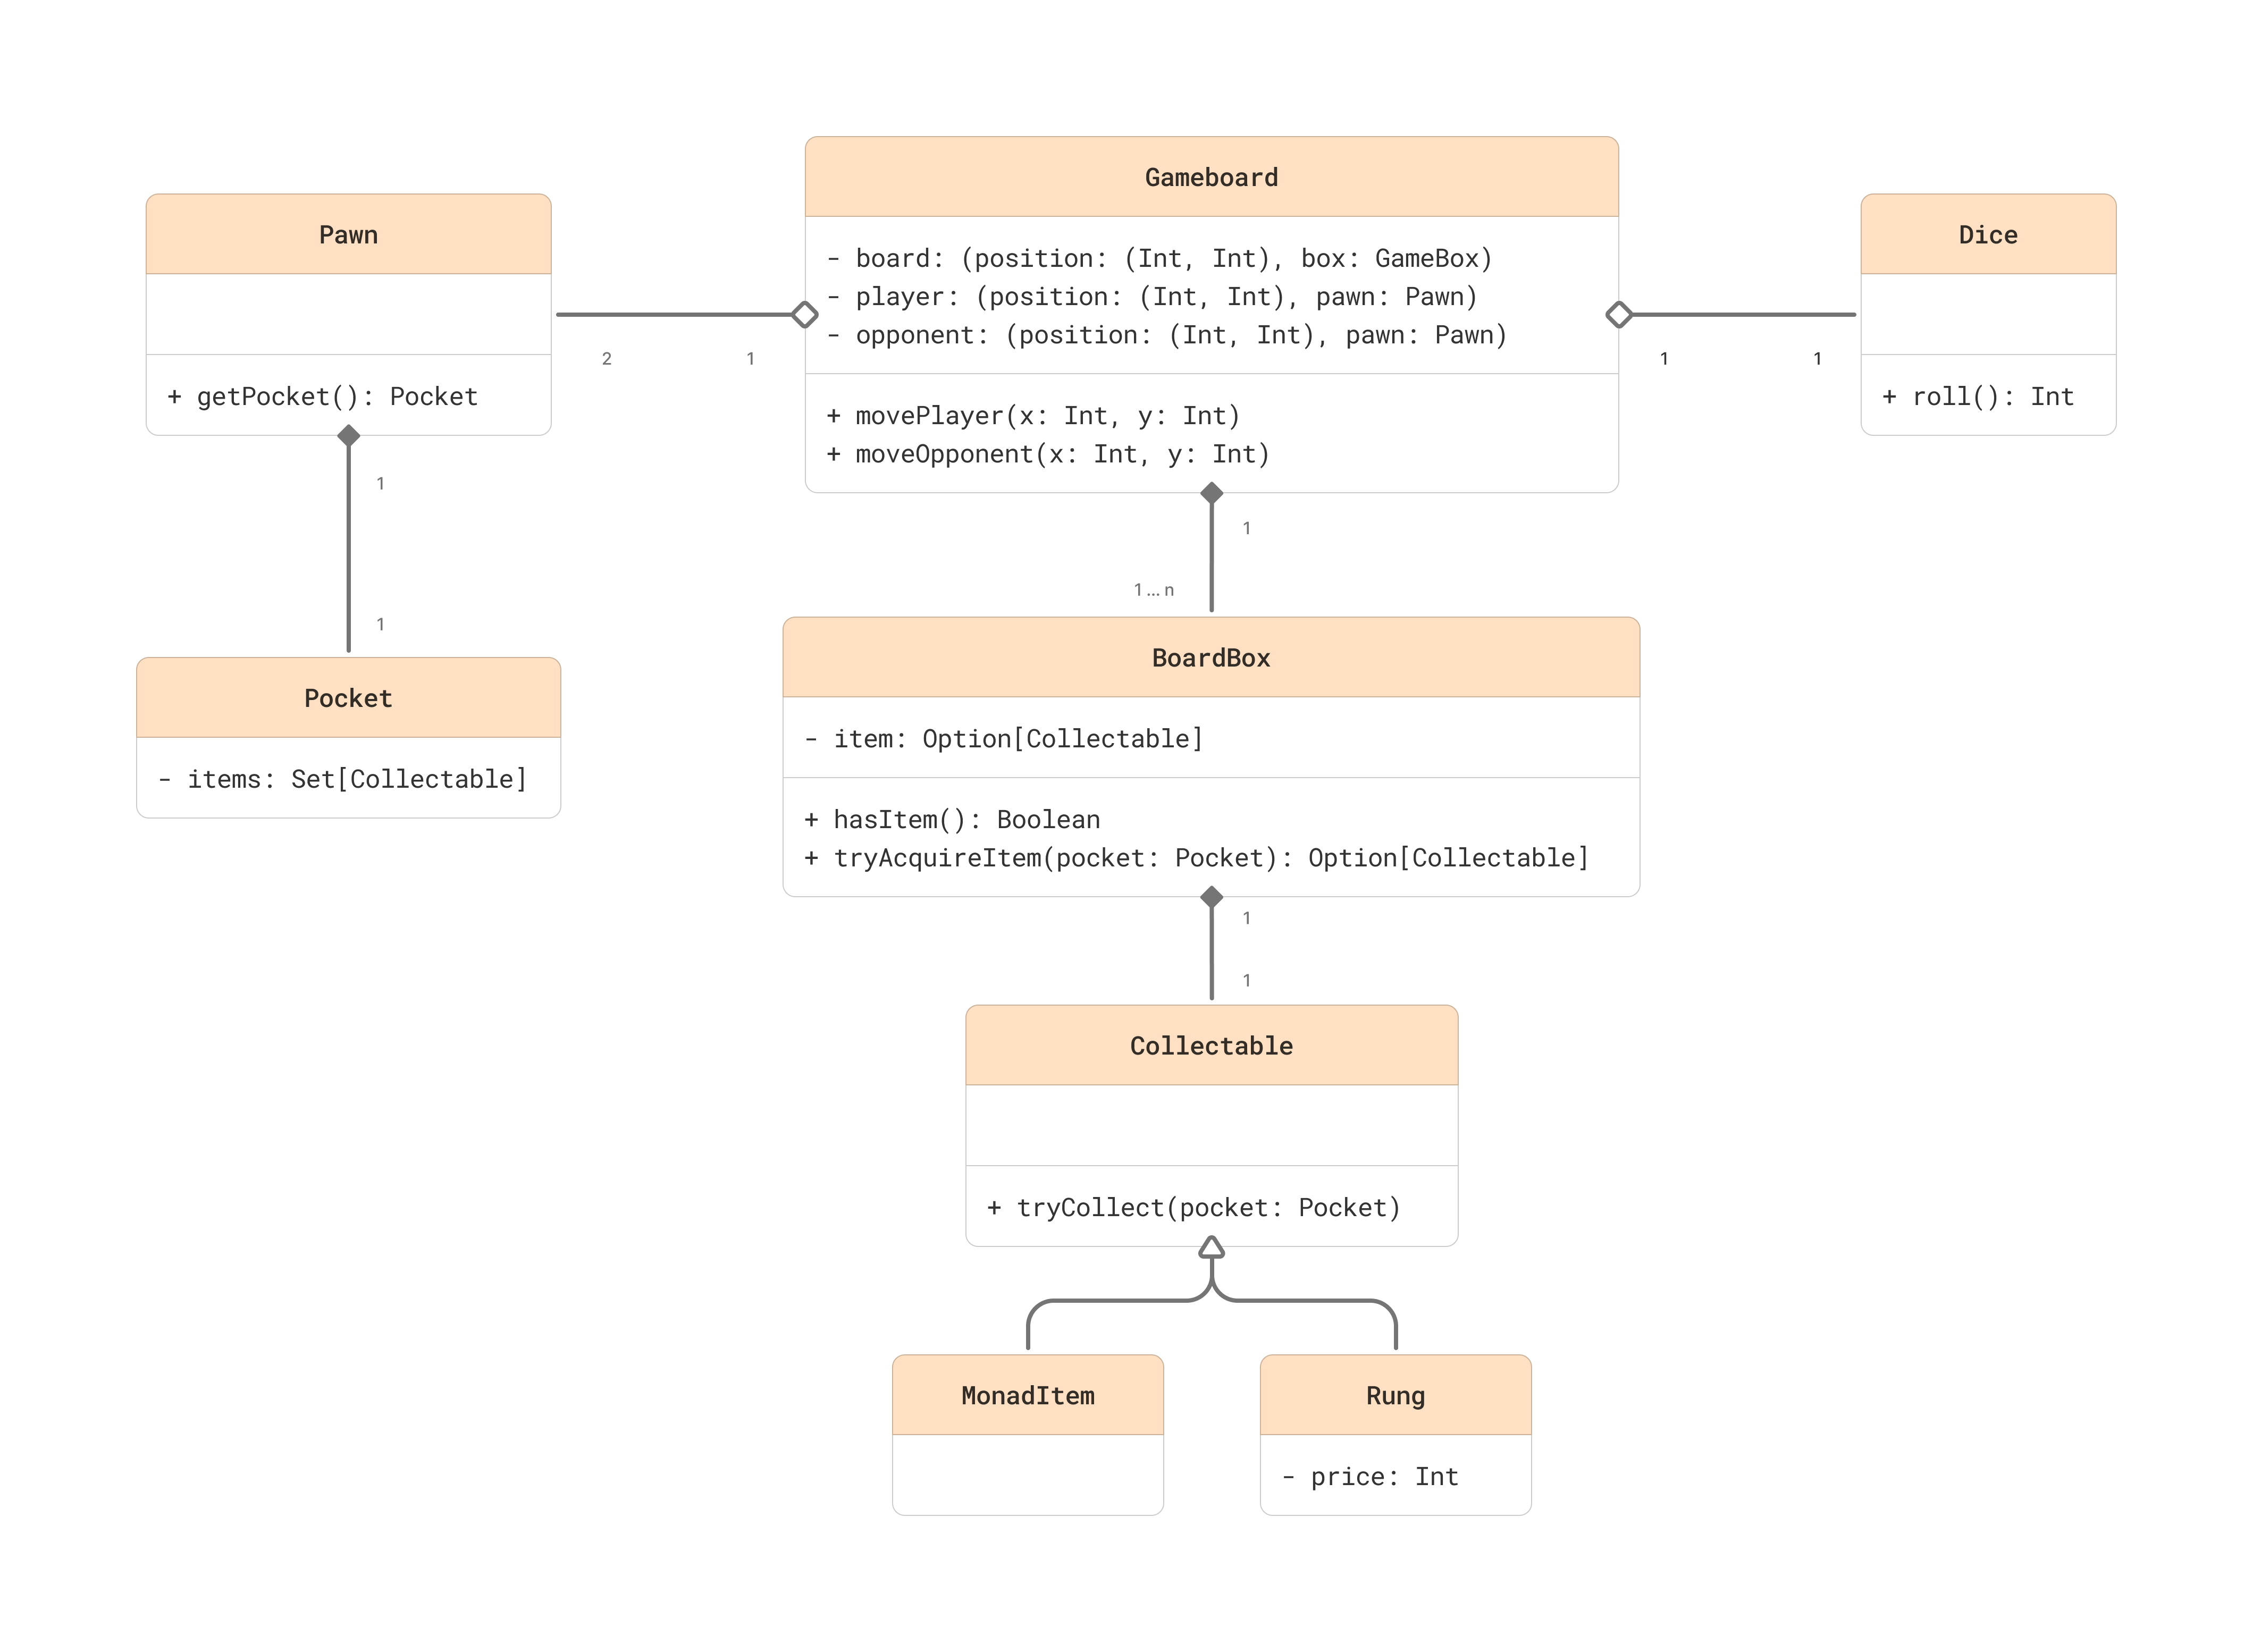
\includegraphics[width=1\textwidth]{figures/domain-class-diagram.png}
\caption{Diagramma delle Classi del Dominio}
\label{fig:domain-class-diagram}
\end{figure}
Approfondiamo le entità modellate nel diagramma delle classi 
a figura \ref{fig:domain-class-diagram}.
\begin{itemize}
    \item \textbf{Gameboard}\par
    Rappresenta il tabellone di gioco. Contiene le caselle 
    su cui si muovono le pedine. Su di esso sono collocati il giocatore
    e l'avversario, entrambi rappresentati dalla propria pedina.
    \item \textbf{Board Box}\par
    Rappresenta una casella del tabellone, che può contenere un oggetto
    collezionabile.
    \item \textbf{Dice}\par
    Rappresenta un dado che può essere lanciato.
    \item \textbf{Pawn}\par
    Rappresenta una pedina di gioco sul tabellone.
    \item \textbf{Pocket}\par
    È il contenitore di oggetti collezionabili raccolti da una pedina.
    \item \textbf{Collectable}\par
    Rappresenta un oggetto collezionabile che può essere raccolto o
    "comprato" scambiandolo con altri oggetti collezionabili.
    \item \textbf{MonadCoin}\par
    È un oggetto collezionabile che può essere usato come moneta di scambio.
    \item \textbf{Rung (Piolo)}\par
    È un oggetto collezionabile che può essere usato per vincere il gioco.
\end{itemize}
\subsubsection{Regole del Gioco}
Per cominciare una partita di Scala Party 
vengono svolte le seguenti inizializzazioni:
\begin{enumerate}
    \item Viene scelto un tabellone di gioco che può essere variabile
    ma deve avere le seguenti caratteristiche:
    \begin{itemize}
        \item Deve essere composto da caselle quadrate, di dimensioni
        uguali.
        \item Ciascuna casella può essere adiacente a un massimo di 4 caselle
        \item Non possono esistere caselle isolate, ovvero non raggiungibili
        muovendosi da una casella ad un'altra adiacente a partire da una qualunque
        casella del tabellone.
    \end{itemize}
    \item Viene posizionato un piolo in una casella casuale del tabellone.
    \item Vengono posizionate dieci monadi in caselle casuali del tabellone.
    \item Viene scelta una casella di partenza su cui posizionare le pedine
    del giocatore e dell'avversario.
\end{enumerate} 
A questo punto, la partita può iniziare e si svolgerà seguendo le seguenti fasi:
\begin{enumerate}
    \item \textbf{Lancio dei dadi per l'ordine dei turni}\par
    Il giocatore e l'avversario lanciano un dado ciascuno. Chi ottiene
    il numero più alto sarà il primo a giocare in ogni ciclo di turni della partita.
    \begin{itemize}
        \item Il dado è un dado standard a 6 facce.
        \item In caso di pareggio tra i due giocatori, il lancio viene ripetuto
    \end{itemize}
    \item \textbf{Turni di gioco}\par
    Ciascun ciclo di turni è composto dal turno del giocatore e da quello dell'avversario.
    Il turno si svolge in questo modo:
    \begin{enumerate}
        \item \textbf{Lancio dei dadi}\par
        Il giocatore di turno lancia uno o due dadi 
        (maggiori dettagli su questo aspetto saranno 
        discussi in seguito) per determinare il numero di passi
        che potrà compiere con la propria pedina.
        \item \textbf{Movimento della pedina}\par
        Il giocatore di turno muove la propria pedina in qualsiasi
        direzione, a seconda del numero di passi ottenuto dal lancio.
        \begin{itemize}
            \item Ad ogni passo, il giocatore può scegliere di spostarsi
            in una qualsiasi casella adiacente.
            \item Durante il movimento, quando il giocatore si sposta
            su una casella che contiene un oggetto collezionabile, 
            questo viene automaticamente raccolto se il giocatore ha
            le risorse necessarie per ottenerlo.
            \item I Collezionabili sono di due tipi:
            \begin{itemize}
                \item \textbf{Monade}\par
                Rappresenta la valuta di scambio del gioco e può essere ottenuta gratuitamente
                \item \textbf{Piolo}\par
                Può essere ottenuto scambiando cinque monadi, maggiori dettagli
                su questo saranno discussi in seguito.
            \end{itemize}
        \end{itemize}
        \item \textbf{Ottenimento del Piolo}\par
        Quando un giocatore di turno si sposta su una casella che contiene un piolo, 
        può ottenerlo solo se ha a disposizione cinque monadi da scambiare. Una volta raccolto il piolo,
        un nuovo piolo viene posizionato in una casella casuale del tabellone, le monadi
        rimaste nel tabellone vengono rimosse e ne vengono aggiunte dieci nuove.
    \end{enumerate}
    Alla fine di ogni ciclo di turni, il giocatore partecipa a un \textbf{Minigioco}.
    Se vince, potrà lanciare due volte il dado nel turno successivo, 
    se invece perde, sarà l'avversario a lanciare due volte il dado.
    \item \textbf{Fine della partita}\par
    La partita termina quando uno dei due giocatori raccoglie 4 pioli,
    e verrà dichiarato vincitore.
    
\end{enumerate}
